\chapter{Measurement of the inclusive \ttbar cross section at \sqrtsRIII}
\label{ch:ttxs}

This chapter describes the measurement of the inclusive \ttbar production cross section at the LHC at the center-of-mass energy of \sqrtsRIII performed as part of this thesis. First, a motivation and overview of the analysis design will be given. Then, object and cut definitions as well as several applied corrections will be explained in detail. Finally, the likelihood fit used to extract the cross section, including all uncertainties, is described and the result discussed.

\section{Introduction}

% motivation: new com energy, possible glimpse at new physics; new run, new calibrations, top physics requires most objects -> good check of performance

% method needs to be tuned for early measurement
% special mention: lepton sf -> can be estimated in situ
% do one fit with and one without

In July 2022, the LHC officially resumed collecting data after a roughly three-year technical stop, thereby starting LHC Run 3. It did so at a new, unprecedented center-of-mass energy of \sqrtsRIII, inviting the experiments to measure energy-dependent physical observables at the new energy frontier.

One important such observable is the inclusive \ttbar production cross section. As mentioned in Ch. \ref{ch:theory}, the top quark has a special place in the standard model as the heaviest known elementary particle, as well as the only colored particle that, due to its short lifetime, does not hadronize. It is thus of importance for many BSM scenarios such as additional Higgs-like bosons, which might couple strongly to the top quark. As such, a measurement of top-related observables at the highest possible energies can be used to test the Standard Model. The inclusive \ttbar cross section, as one of the simplest top quark observables, is thus well suited for a first such measurement at the new center-of-mass energy.

Simultaneously, restarting such a large experiment as the CMS detector after a three-year technical stop poses many experimental challenges. Due to the change in energy, as well as physical changes in the accelerator and detector, most calibrations and corrections used to correctly describe the recorded data in simulation need to be re-derived and validated. An early measurement of the inclusive \ttbar cross section is well suited to cross-check this: Because of the decay chain of the top quark, a top-related measurement involves several of the different objects reconstructed at CMS, as described in Ch. \ref{sec:methods:reco}, enabling a check of a wide landscape of calibrations.

The measurement described in this chapter was designed specifically with these motivations in mind, and as such exhibits several novel features. Firstly, it combines events from both the dilepton and \ljets decay channels of \ttbar, categorized by lepton flavor content, combining the higher statistics of the \ljets channel with the high purity of the \emu channel and allowing to constrain uncertainties on the lepton identification efficiency directly from the data. This is done using a maximum likelihood fit to the event yields in the different categories, with experimental and theoretical uncertainties treated as nuisance parameters.

Secondly, the events are additionally categorized by their number of b-tagged jets, which similarly allows for an in-situ measurement of the b-tagging efficiencies. This prevents the need to wait for external b-tagging calibrations, making for the earliest possible measurement.

\section{Datasets and event selection}

In this section, the choice of datasets for experimental data and for simulation, as well as the choice of triggers, is described. Following that, the object and event selection procedure is outlined and several event categories, to be used in the likelihood fit~\ref{sec:ttxs:fit}, are defined. 

\subsection{Datasets}
\label{sec:ttxs:datasets}

\paragraph{Experimental data.}
The measurement is performed on data recorded during the period between July 27\textsuperscript{th} and August 02\textsuperscript{nd} 2022 (part of Era C of year 2022), corresponding to an integrated luminosity of $1.20 \pm 0.07$ pb. This amount of data is chosen as a balance between sensitivity and speed for the early measurement: It roughly corresponds to the point where data statistics no longer significantly limit the measurement uncertainty, while at the same time it is not required to study calibrations at different beam and detector conditions (e.g. average pileup, which changed during the different eras of 2022).

% TODO luminosity measurement

Both single-lepton and dilepton triggers were used to select events used in this measurement during detector operation, identifying leptons in the range of $\abseta < 2.5$. The \pt requirements of the triggers are summarized in Tab.~\ref{tab:ttxs:triggers}.

\begin{table}
    \centering
    \begin{tabular}{c|c}
        Trigger & Lepton requirement \\
        \hline
        single-e & e($\pt > 32$ GeV) \\
        single-$\mu$ & $\mu$($\pt > 27$ GeV) \\
        ee & e($\pt > 23$ GeV) and e($\pt > 12$ GeV) \\
        $\mu\mu$ & $\mu$($\pt > 17$ GeV) and $\mu$($\pt > 8$ GeV) \\
        e$\mu$ & e($\pt > 23$ GeV) and $\mu$($\pt > 8$ GeV)  or \\
        & e($\pt > 12$ GeV) and $\mu$($\pt > 23$ GeV) \\
    \end{tabular}
    \caption{Trigger definitions used for the \ttbar cross section measurement. The leptons are required to be isolated and in the pseudorapidity range  $\abseta < 2.5$.}
    \label{tab:ttxs:triggers}
\end{table}

\paragraph{Simulation.}
To compare the data with predictions, Monte Carlo (MC) simulation is used to simulate both the \ttbar signal as well as most important background processes, specifically single-top quark production in the $t$-channel, associated tW-production, Z+jets production, W+jets production, and diboson (WW, WZ and ZZ) production. The MC generator \textsc{Powheg v2}~\cite{Powheg:2004, Powheg:2007, Powheg:2010} is used to generate \ttbar, single-top, and tW events at next-to-leading order (NLO) in perturbative QCD, while the generators \textsc{MadGraph5\_aMC@NLO}~\cite{MG5aMCatNLO:2014} and \textsc{Pythia 8}~\cite{Pythia:2015} are used to generate Z+jets/W+jets and diboson events, respectively, at leading order (LO). For $t$-channel single-top, specifically, \textsc{MadSpin} is used to simulate the top decay.

All of the generated events are interfaced to \textsc{Pythia 8} for parton showering and hadronization, using the MLM prescription in the case of the samples produced with \textsc{MadGraph}, and further processed in a full simulation of the CMS detector using \textsc{Geant 4}~\cite{GEANT4:2002}. The proton structure in the matrix element calculation is described by the NNPDF3.1 parton distribution function (PDF) set at NNLO. Note that another background contribution, from QCD events with fake or non-prompt leptons, is not simulated, but estimated from data (see sec. ??).

Theoretical predictions, as well as the measured integrated luminosity, are used to normalize the cross sections of the signal and background samples as follows: The \ttbar signal, computed at NNLO+NLLL in QCD, gives a value of \xsecpred, which is also used as prediction for comparison with the SM. For the other backgrounds, the following orders in QCD and methods or programs are used: \textsc{MCFM}~\cite{Campbell:2020fhf} (NNLO) for single-top, \textsc{DYTurbo}~\cite{Camarda:2019zyx} (NNLO) for W+jets and Z+jets, \textsc{Matrix}~\cite{Grazzini:2017mhc} (NLO) for diboson, and Ref. \cite{Kidonakis:2021vob} (NNLO) for tW.




\subsection{Object definition}
\label{sec:ttxs:objects}

\paragraph{Leptons.}

Electrons or muons are considered for the analysis if they have $\pt > 10$ GeV and $\abseta < 2.4$. For electrons, the range $1.44 < \abseta < 1.57$, corresponding to the transition region between barrel and endcaps in the ECAL, is removed. Furthermore, additional identification criteria (ID) are applied to remove non-prompt or fake (i.e. wrongly reconstructed) leptons and enrich the selection with \ttbar events as such:

For electrons, the "tight" working point of the cut-based ID described in \citere{CMS:EGM-17-001} is applied, which includes information from both the details of the electromagnetic shower in the ECAL and the track, as well as the matching between the two. It also includes a requirement for the electron to be isolated from other particles such as hadrons, which is implemented in the form of the relative isolation variable. It is defined as the scalar \pt sum of all particles in a cone around the lepton in question, divided by the lepton \pt. Here, $\Delta R = \sqrt{(\Delta \eta)^2 + (\Delta \phi)^2} < 0.3$ is used for the radius of the cone. Additional corrections accounting for pileup particles are applied.

For muons, a similar cut-based ID is used as described in \citere{CMS:MUO-16-001}, also at the tight working point. Here, criteria on the compability of tracks in the innter tracker, the muon detectors and the reconstructed primary vertex are employed. Again, a cut on the relative isolation variable is used, defined equivalently but with a cone size of $\Delta R < 0.4$.

\paragraph{Jets.}

The anti-$k_T$ algorithm is used to cluster reconstructed particles into jets with a distance parameter of 0.4. In order for a jet to be considered, it is required to have $\pt > 30$ GeV and $\abseta < 2.4$, and jets overlapping with any considered leptons (i.e. fulfilling the above criteria) are removed. %Again, additional ID criteria, based on the fractions of \pt originating from neutral hadron, charged hadron and electromagnetic jet constituents, are used to reject 

\paragraph{Tagging of b jets.}

A special role is played by jets originating from the showering and hadronization of b quarks. Naively, two such jets are expected per \ttbar event from the two top decays, although in practice one or both jets may fall out of acceptance of the detector or otherwise not get identified. Correctly tagging these jets as such can greatly improve signal purity by cutting away backgrounds such as Z+jets, W+jets and QCD multijet events.

Here, the \textsc{DeepJet} algorithm is used to tag b jets, which is based on a deep neural network (DNN) classifier~\cite{DeepJet:2020,CMS:BTV-16-002}. A working point with an identification efficiency of more then 75 \% is used, with misidentification rates of around 17 \% for c jets and around 1 \% for other jets (i.e. from light quarks or gluons).

\subsection{Channel definition}
\label{sec:ttxs:channels}

Events are selected with either one or two leptons, corresponding to the dilepton and \ljets decay channels of \ttbar, respectively. They are categorized into lepton channels by their lepton flavor content, and additional requirements are applied for the different channels. 

\paragraph{Dilepton channels.}

Events with exactly two leptons, required to have opposite electric charge, are sorted into three dilepton channels (\emu, ee, and $\mu\mu$). The presence of at least one jet is required, and in the same-flavor channels (ee and $\mu\mu$), at least one jet is required to be b tagged in order to reject Z+jets and QCD multijet background. In the much purer \emu channel, on the other hand, events without b tags are retained to later help constrain the b tagging efficiency in the fit to data.

In order to reject even more Z+jets background, events in the same-flavor channels with an invariant dilepton mass of $| \mll - m_Z | < 15$ GeV, where $m_Z$ is the Z boson mass, are removed.

\paragraph{\ljets channels.}

Events with exactly one lepton are sorted into the e+jets or $\mu$+jets channels based on their flavor. At least three jets are required, of which at least one needs to be b tagged. Note that regardless of these selections, there is still non-negligible background from QCD multijet events where the lepton is non-prompt or fake, which will be estimated from data (see sec. ??).

\paragraph{\pt requirement.}

In all channels, the considered leptons are required to have $\pt > 35$ GeV. This requirement is needed in the \ljets channels in order to stay above the single-lepton trigger \pt thresholds (compare Tab. \ref{tab:ttxs:triggers}). In this measurement, the choice is made to apply the same \pt requirement also both leptons in the dilepton channels to ensure consistency between the lepton definitions. This is done to help constrain the lepton ID scale factors using the combination of lepton flavor channels, which otherwise might not be accurate since the scale factors for different lepton definitions might differ (see sec. ??). Especially, it opens up the possibility to extract a result on the cross section without any prior knowledge on the lepton ID efficiencies, which was done in the first published version of this analysis \cite{CMS:TOP-22-012-PAS} and is included in this thesis as a cross-check (see sec. ??).

\paragraph{b tag and jet categorization.}

In practice, the efficiency of the b tagging algorithm used might be different between simulation and data, necessitating a correction to prevent bias. In this analysis, this efficiency is measured simultaneously with the cross section directly in the data. To do so, the lepton flavor channels are additionally split into categories based on the number (exactly 0, 1, or 2) of b tagged jets. Since only the \emu channel allows events with 0 b tags, this results in 11 categories total.

In order to increase possible separation between \ttbar signal and background, the selected events are finally coarsely binned into the number of accepted jets for the eventual fit, giving a total number of 40 bins.

\section{Corrections}
\label{sec:ttxs:corrections}

While the simulation used in CMS tries to model as many physics and detector effects as possible, in practice it should always be expected that not all observables agree with the experimental data perfectly. This is especially true for an early analysis such as this, as the detector conditions might have changed significantly during the long shutdown between LHC Runs 2 and 3, and the simulation had not been recalibrated at the time of the measurement. 

Because of this, the analysis setup is designed to either directly measure or cross-check as many required experimental calibration and correction factors as possible. This includes pileup corrections, efficiency scale factors for triggers, electrons, muons and b tags, as well as jet energy corrections, all of which are briefly described in this section.

In addition to these experimental corrections, background processes might also be imperfectly described by the simulation because of theoretical shortcomings. In this case, ways have to be found to correct them, which might also involve experimentally measuring them. Here, two such cases are relevant and will be presented in the latter half of this section: The Z+jets background in the dilepton channels and presence of b tagged jets, for which the normalization is taken from data; and the QCD background in the \ljets channels, which uses a fully data-driven estimation and foregoes simulation entirely.

\subsection{Experimental corrections}
\label{sec:ttxs:scalefactors}

\paragraph{Pileup reweighting.}

The simulation samples used in this analysis were generated before the start of Run 3 data taking using a projected estimate of the average pileup. As a result, the pileup distribution in the simulation does not match the one observed in data, which could influence mostly jet-related variables such as the number of jets and the jet \pt.

Since at the time of the measurement, no theoretical calculations for the correct pileup distribution were available, an experimental approach was taken. Three experimental observables that are strongly correlated with pileup were identified: the number of good primary vertices, the mean energy density measured in the calorimeter, and the mean energy density measured in the tracker. A binned reweighting from simulation to data is derived for each observable based on our full data sample, and the average of the three weights is applied to the simulation going forward to achieve approximate agreement in all variables with the available statistics. The distributions before and after reweighting can be seen in Fig. ??.

\paragraph{Trigger scale factors.}

One of the efficiencies that might need to be corrected for in the simulation is that of the triggers, i.e. the probability for an event falling into the selection phase space to be triggered by the low- and high-level triggers. It should be noted that, while both dilepton and single-lepton triggers are used for the measurement, the single-lepton triggers by far dominate the selected event count due to the high \pt thresholds required, and so the efficiency is measured for the single-lepton triggers only for simplicity.

The measurement is performed by the so-called tag-and-probe (T\&P) method, using $\mathrm{Z} \rightarrow \mathrm{e^+ e^-}$ and $\mathrm{Z} \rightarrow \mathrm{\mu^+ \mu^-}$ events. They are selected using the same definitions presented above, including the lepton identification, except for requiring their invariant mass to fulfill $| \mll - m_Z | < 20$ GeV. At least one of the leptons is required to pass the relevant single-lepton trigger and is then designated the tag, while the other lepton might or might not pass the trigger and is designated the probe. Assuming the probability for the two leptons to pass the trigger to be independent of each other, the trigger efficiency, given by probability of the probe to pass, can be written as

\begin{equation}
    \epsilon_{\mathrm{tr}} = \frac{N (\text{Probe passes})}{ N (\text{Probe passes}) + \frac{1}{2} N (\text{Probe fails}) }
\end{equation}

where $N$ is the observed event yield, and the combinatoric factor $\frac{1}{2}$ comes from the fact that either one or the other lepton can fail to pass the trigger. 

The efficiency is measured in this way in coarse bins of lepton \pt and \abseta, seperately for muons and electrons, in both simulation and experimental data. It is then applied to simulation in the following way: For \ljets events, a simple ratio $\epsilon_{\mathrm{tr,data}} / \epsilon_{\mathrm{tr,sim}}$ is applied to each simulation event as a scale factor, while for dilepton events, the fact only one lepton needs to pass the single-lepton trigger needs to be taken into account. This leads to a per-event efficiency given by

\begin{equation}
\label{eq:ttxs:triggersf}
    \epsilon_{\mathrm{tr,\ell \ell}} = \epsilon_{\mathrm{tr,\ell 1}} + \epsilon_{\mathrm{tr,\ell 2}} - \epsilon_{\mathrm{tr,\ell 1}} \epsilon_{\mathrm{tr,\ell 2}}
\end{equation}

where $\epsilon_{\mathrm{tr,\ell 1}}$ and $\epsilon_{\mathrm{tr,\ell 2}}$ are the efficiencies of the two leptons, respectively. Again, the ratio of this event efficiency in data and simulation is applied to the simulation.

\paragraph{Lepton scale factors.}

Similarly to the triggers, the reconstruction and identification of leptons can exhibit different efficiencies between simulation and data. Here, they are combined into a single lepton efficiency with an associated scale factor (i.e. ratio between data and simulation).

Two orthogonal approaches are taken with respect to this: In the first approach, the efficiencies are measured with a similar tag-and-probe method as for the triggers, and the simulation is corrected to the data. This is the standard approach commonly taken in CMS, and will be used in the figures presented in this thesis unless stated otherwise.

In the second, alternative, approach, on the other hand, no correction to the simulation is made, and instead the lepton efficiencies in data in the selection phase space are measured simultaneously with the cross section using the likelihood fit. This will be further described in sec. ??.

\paragraph{b tagging scale factors.}

The performance of b tagging algorithms, including the \textsc{DeepJet} algorithm used here, is well-known to have differences between simulation and data, and will need correction factors. This is especially true since the multivariate classifier underlying \textsc{DeepJet} had at the time of the measurement not been re-trained on Run 3 data, and the calibration from Run 2 was used instead.

Analogously to the alternative approach to the lepton scale factors detailed above, the b tagging correction is not applied to the simulation in this analysis, but instead measured simultaneously with the \ttbar cross section in a single likelihood fit, as described in sec. ??.

\paragraph{Jet energy corrections.}

Another observable that often differs significantly between observed data and simulation is the measured energy response of the jets. It is usually corrected both by theoretical means, e.g. accounting for detector resolution, and by empirical methods, i.e. comparing simulation to data for well-known resonances like the Z boson. Unlike the other scale factors mentioned here, the jet energy correction (JEC) is not measured as part of this thesis, and instead centrally provided by CMS following the methods of Ref. ??. 

\subsection{Data-driven backgrounds}
\label{sec:ttxs:datadriven}

\paragraph{QCD background.}

A significant background contribution in the \ljets channels, especially in the categories with only one b tag, is given by QCD multijet events with one reconstructed lepton. The lepton in question might be non-prompt, meaning from radiation or hadronization, or it might be fake, i.e. a different particle (such as a photon or pion in the case of electrons) misidentified as a lepton. 

It is often not practical to estimate this background using MC simulation as is done for the other backgrounds in this analysis. The reason is that, due to the large cross section of QCD multijet events at the LHC but low ratio of events with a fake or non-prompt lepton, very large MC datasets are needed to achieve significant statistics in the selected phase space, which would require excessive computing power. In addition to that, especially fake leptons are not certain to be described well by the simulation.

Instead, a fully data-driven approach is taken to estimate the QCD background. For this, several control regions (CRs), orthogonal to the signal region (SR) are defined. In the first CR, the same cuts as in the SR are applied, except that the requirement for the single lepton to be isolated from other particles (see sec. \ref{sec:ttxs:objects}) is inverted. It is expected that QCD events that fall in either this CR or the SR show similar shapes in observable distributions, as long as said observables are uncorrelated with the lepton isolation. Thus, the shape of the QCD background can be extracted from the CR and applied in the SR.

In order to fix the normalization of the QCD background, a second region is defined. It again contains events that pass the selection in the SR, except for requiring exactly one jet (as opposed to at least three jets in the SR). These events are enriched with QCD events and contain negligible amounts of \ttbar signal. They are used to measure the ratio $f_{\mathrm{fake}}$ of QCD events that pass or fail the lepton isolation requirement, given by

\begin{equation}
    f_{\mathrm{fake}} = \frac{ N_{\text{SR, 1 jet}}^{\text{data}} - N_{\text{SR, 1 jet}}^{\text{MC}} }{ N_{\text{CR, 1 jet}}^{\text{data}} - N_{\text{CR, 1 jet}}^{\text{MC}} }
\end{equation}

where $N_{\text{SR, 1 jet}}$ and $N_{\text{CR, 1 jet}}$ denote 1-jet-events that pass and fail the lepton isolation requirement, respectively. Here, this ratio is measured in coarse bins of lepton \pt and \abseta to accurately model lepton-related distributions.

The full distribution of the QCD background for any observable can then in principle be written as

\begin{equation}
    N_{\text{SR}}^{\text{QCD}} = ( N_{\text{CR}}^{\text{data}} - N_{\text{CR}}^{\text{MC}} ) \times f_{\mathrm{fake}}
\end{equation}

In practice, this is complicated by the fact that \ttbar signal might be present in the CR defined by the lepton isolation, whose cross section is not known \textit{a priori}. A modified method to correct for this is given in Appendix ??.

\paragraph{Z+jets background.}

In contrast to the QCD background, the Z+jets background can in general be well described by MC simulation. However, in the phase space used in the analysis, there can be problems related to the b tag requirement. For Z+jets events, b jets are only generated at the matrix element level at higher orders in perturbative QCD, and might thus not be perfectly modeled compared to observed data. This in turn could influence the acceptance of Z+jets events, leading to an incorrect normalization in events with one or more b tags.

Here, a data-driven normalization is derived for Z+jets events with one or two b tags in the dilepton channels. This is important especially in the same-flavor channels, where Z+jets is a dominant background.

The normalization is derived using a CR in which the cut on \mll is inverted, i.e. in events with $| \mll - m_Z | < 15$ GeV, which are strongly enriched in Z+jets contributions. It is assumed that the Z+jets contribution in the \emu channel (which stems mostly from $\mathrm{Z} \rightarrow \tau \tau$ events) is negligible compared to the ee and $\mu \mu$ channels, and that all other backgrounds (including \ttbar) are approximately equal in the three dilepton channels in the sense that their differences are small compared to the Z+jets event yield. Then, said Z+jets yield in the CR in the same-flavor channels can be estimated directly from data as

\begin{equation}
\label{eq:ttxs:zjets_yield}
    N_{\mathrm{ee / \mu\mu}}^{\mathrm{Z+jets}} = N_{\mathrm{ee / \mu\mu}}^{\mathrm{data}} - \frac{1}{2} N_{\mathrm{\emu}}^{\mathrm{data}} k_{\mathrm{ee / \mu\mu}}
\end{equation}

where $N_{\mathrm{\ell \ell}}^{\mathrm{data}}$ refers to the number of observed events in the CR for the respective channel, and $k_{\mathrm{ee}} = k_{\mathrm{\mu\mu}}^{-1} = \sqrt{N_{\mathrm{ee}}^{\mathrm{data}} / N_{\mathrm{\mu\mu}}^{\mathrm{data}}}$ is a efficiency factor to correct for the different acceptance of electrons and muons.

To translate this yield from the CR to the SR, the ratio $\Rinout = N_{\mathrm{CR}}^{\mathrm{Z+jets}} / N_{\mathrm{SR}}^{\mathrm{Z+jets}}$ (referring to \textit{inside} and \textit{outside} of the Z window) of event numbers between those two regions has to be estimated. This is done using the MC simulation. However, since this ratio might by itself be mismodeled, it is not directly taken from the simulation. Instead, events with 0 b tags (not considered in the main measurement in the same-flavor channels) are used to construct to construct a more loose assumption, given by

\begin{equation}
    \frac{  \Rinout^{\text{data}} ( \geq \text{1 b tag} ) } { \Rinout^{\text{MC}} ( \geq \text{1 b tag} ) } = \frac{  \Rinout^{\text{data}} ( \text{0 b tags} ) } { \Rinout^{\text{MC}} ( \text{0 b tags} ) }
\end{equation}

This equation in essence means that the \textit{ratio of ratios} in data and MC is independent of the number of b tags. By rearranging it properly and using eq. \ref{eq:ttxs:zjets_yield} for the number of Z+jets events, a normalization scale factor from simulation to data in the SR is derived and applied per lepton flavor channel.

\section{Control distributions}
\label{sec:ttxs:control}

In this section, the agreement between simulation and data in several control distributions is presented, shown in \Cref{fig:ttxs:control_em,fig:ttxs:control_eemm,fig:ttxs:control_ljets}. All corrections described in the previous section are applied in these figures.

\begin{figure}[!p]
\centering
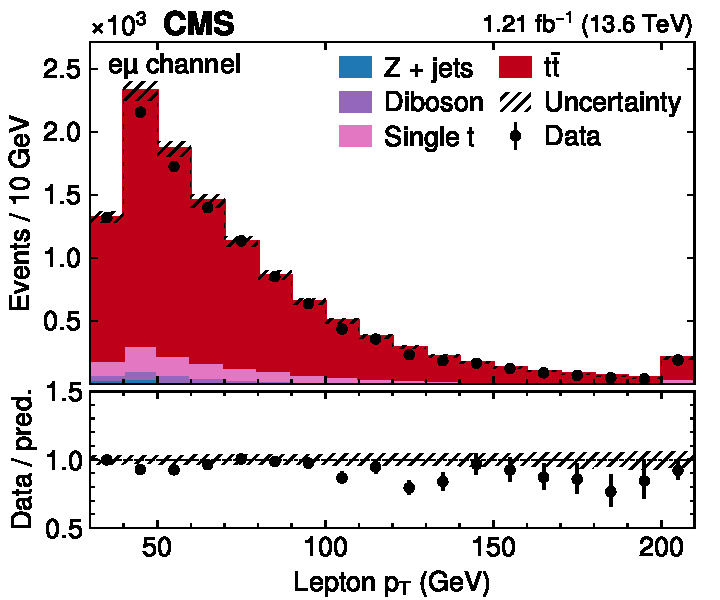
\includegraphics[width=0.49\textwidth]{figures/ttxs/lep_pt_em.pdf}
\hfill
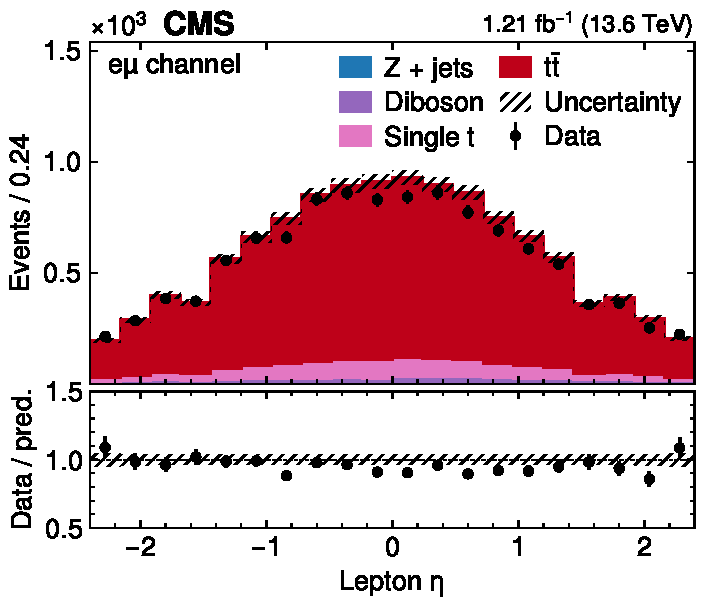
\includegraphics[width=0.49\textwidth]{figures/ttxs/lep_eta_em.pdf}
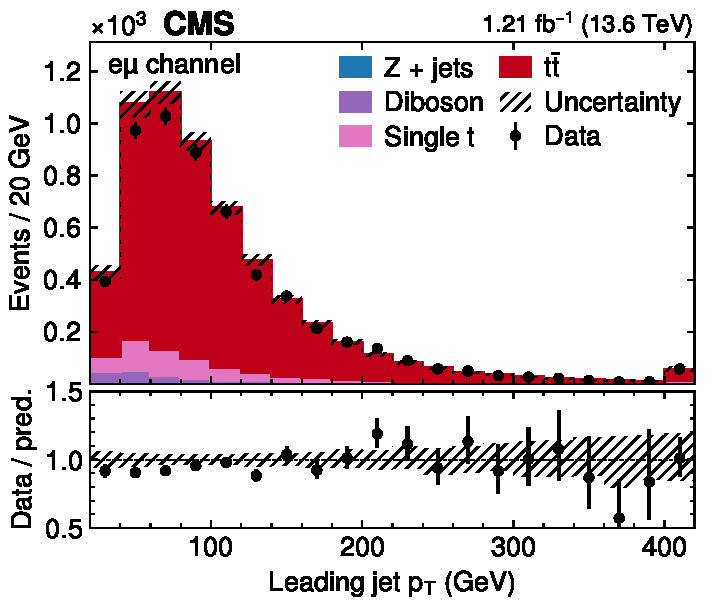
\includegraphics[width=0.49\textwidth]{figures/ttxs/1st_jet_pt_em.pdf}
\hfill
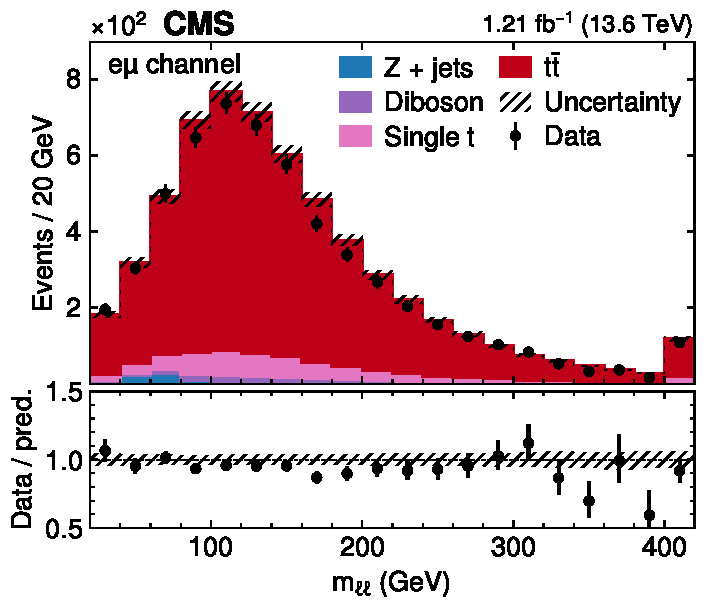
\includegraphics[width=0.49\textwidth]{figures/ttxs/mll_em.pdf}
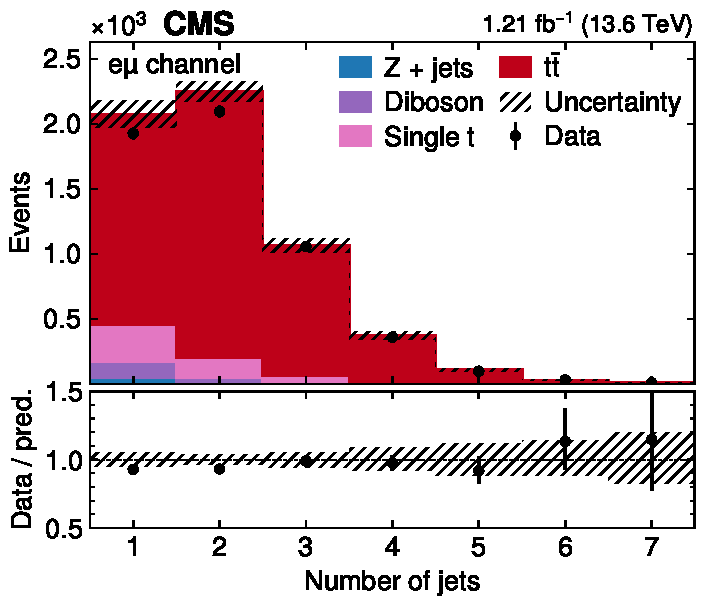
\includegraphics[width=0.49\textwidth]{figures/ttxs/njet_em.pdf}
\hfill
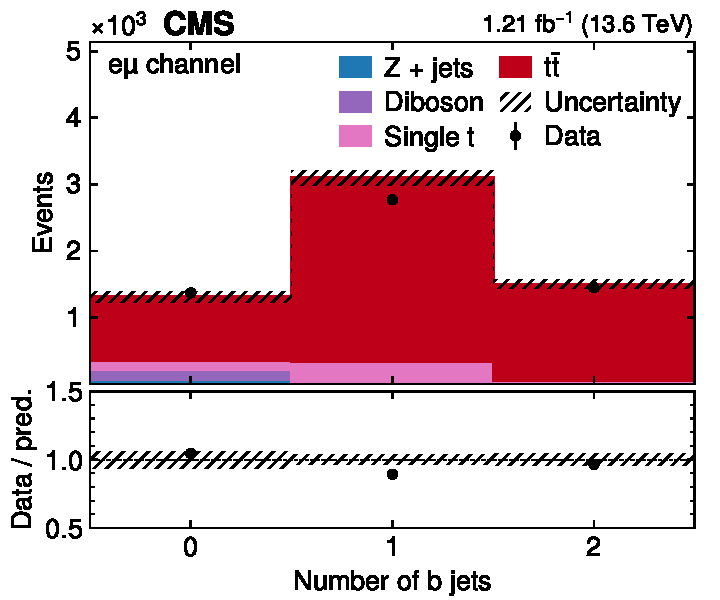
\includegraphics[width=0.49\textwidth]{figures/ttxs/nbtag_em.pdf}
\caption{
    \textbf{Control distributions in the \emu channel.} Shown are (from top left to bottom right) the distributions of \pt of both leptons, \abseta of both leptons, \pt of the leading jet, the invariant lepton mass \mll, the number of jets and the number of b jets. All figures show both data (black dots) and different simulated background processes (colored bars). For the latter, all corrections described in sec.~\ref{sec:ttxs:corrections} are applied, and the shaded area covers both statistical and systematic uncertainties. 
}
\label{fig:ttxs:control_em}
\end{figure}

\begin{figure}[!p]
\centering
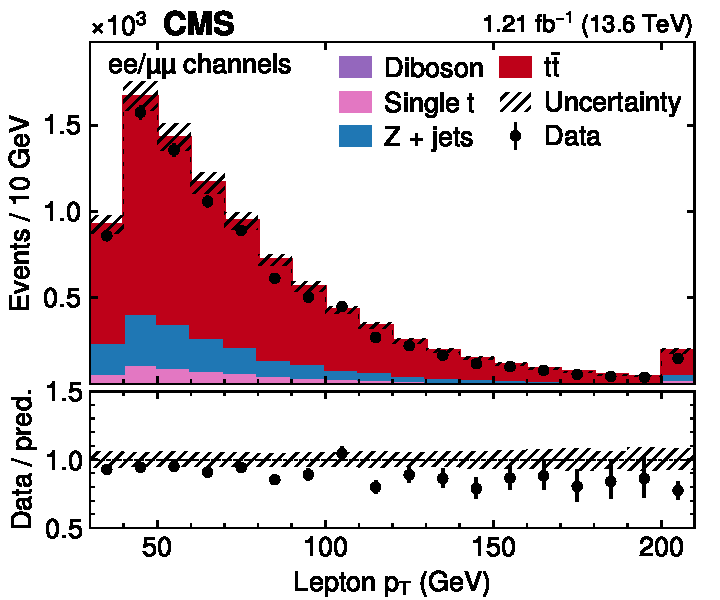
\includegraphics[width=0.49\textwidth]{figures/ttxs/lep_pt_eemm.pdf}
\hfill
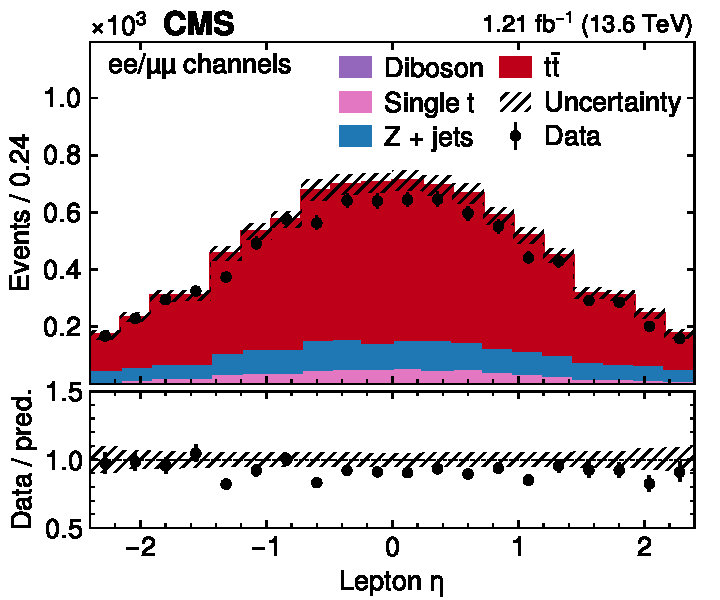
\includegraphics[width=0.49\textwidth]{figures/ttxs/lep_eta_eemm.pdf}
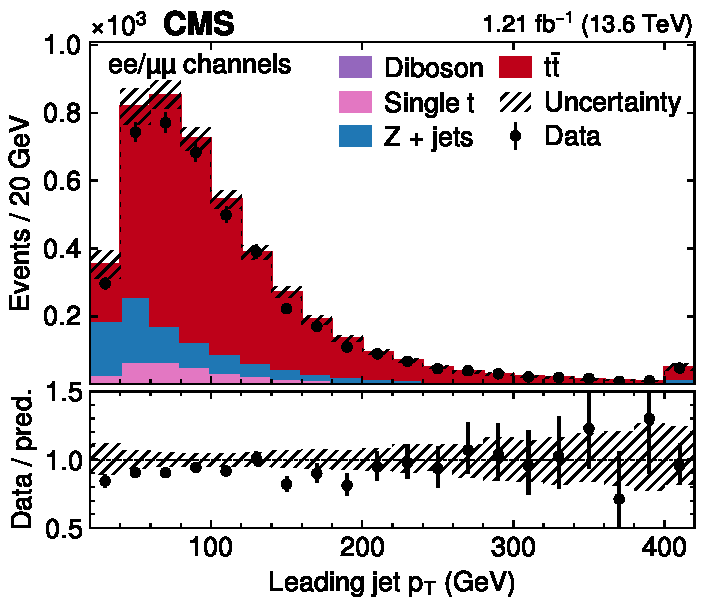
\includegraphics[width=0.49\textwidth]{figures/ttxs/1st_jet_pt_eemm.pdf}
\hfill
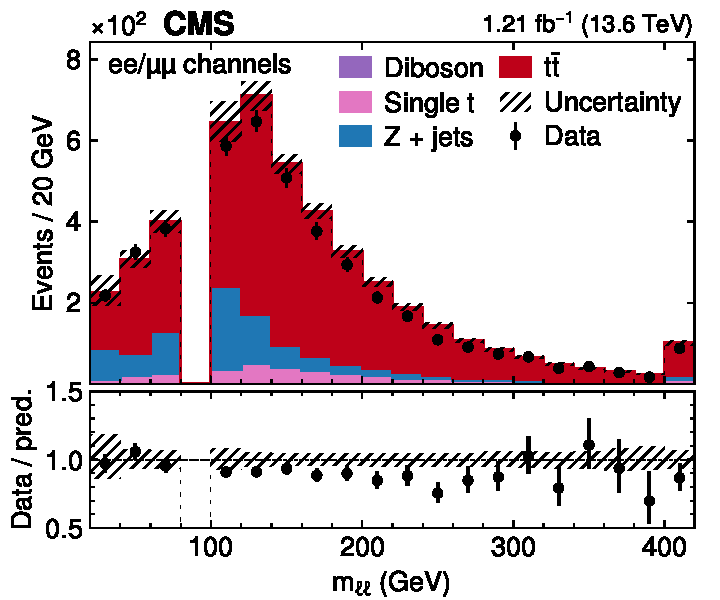
\includegraphics[width=0.49\textwidth]{figures/ttxs/mll_eemm.pdf}
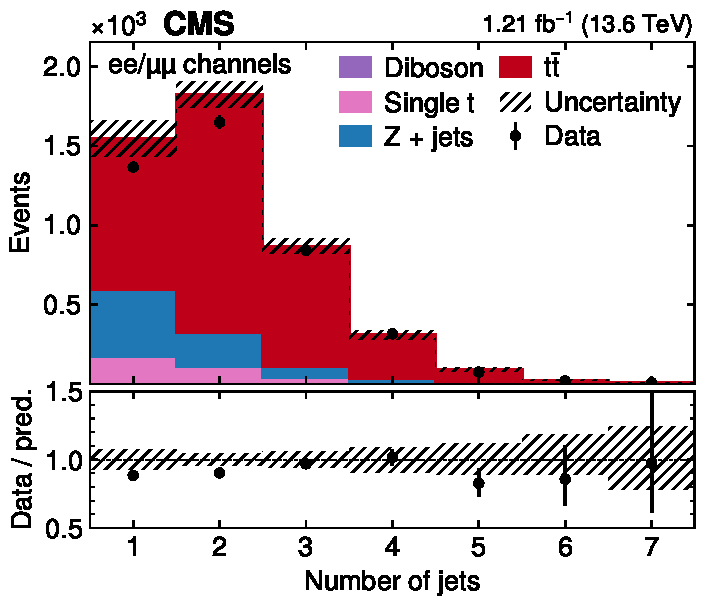
\includegraphics[width=0.49\textwidth]{figures/ttxs/njet_eemm.pdf}
\hfill
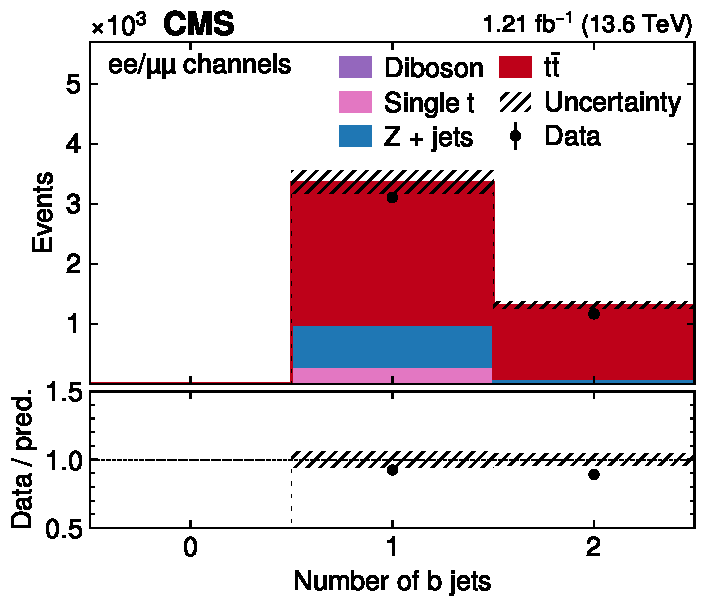
\includegraphics[width=0.49\textwidth]{figures/ttxs/nbtag_eemm.pdf}
\caption{
    \textbf{Control distributions in the \ee and \mumu channels.} The distributions are shown in the same manner as in Fig.~\ref{fig:ttxs:control_em}.
}
\label{fig:ttxs:control_eemm}
\end{figure}

\begin{figure}[!p]
\centering
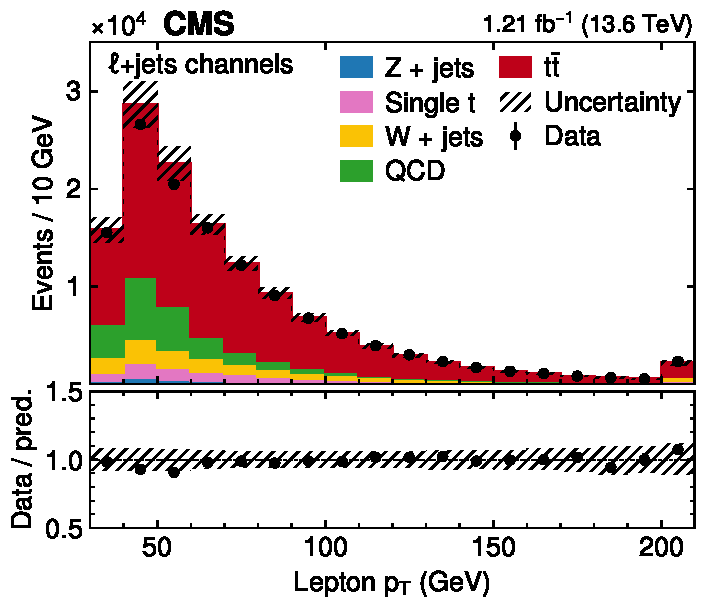
\includegraphics[width=0.49\textwidth]{figures/ttxs/lep_pt_lj.pdf}
\hfill
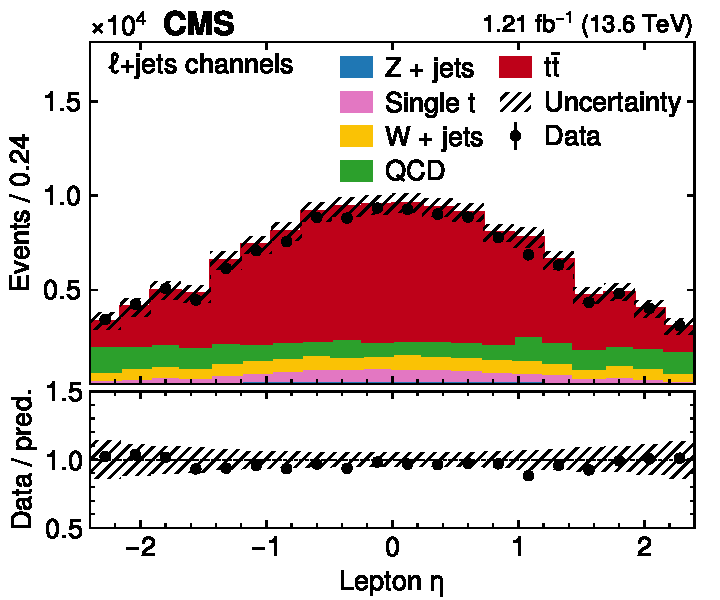
\includegraphics[width=0.49\textwidth]{figures/ttxs/lep_eta_lj.pdf}
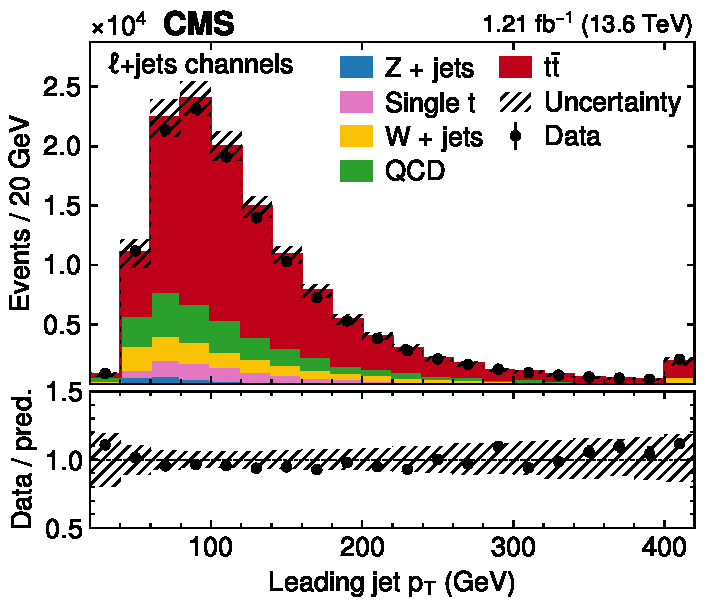
\includegraphics[width=0.49\textwidth]{figures/ttxs/1st_jet_pt_lj.pdf}
\hfill
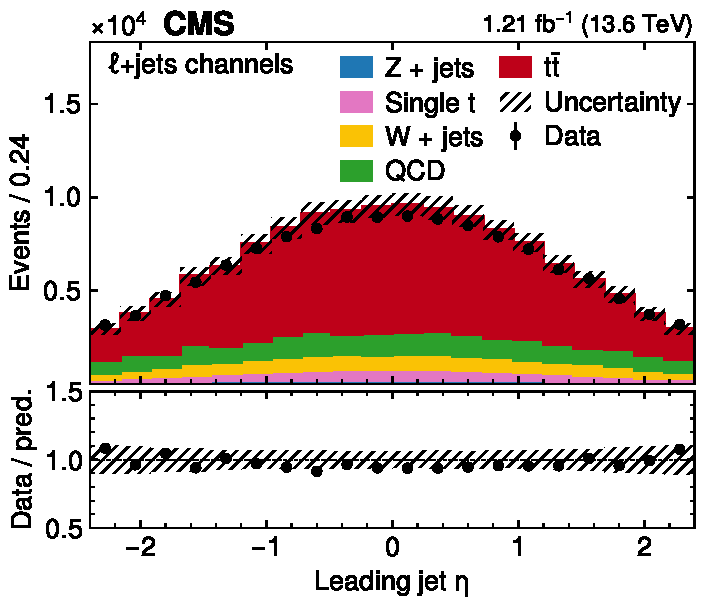
\includegraphics[width=0.49\textwidth]{figures/ttxs/1st_jet_eta_lj.pdf}
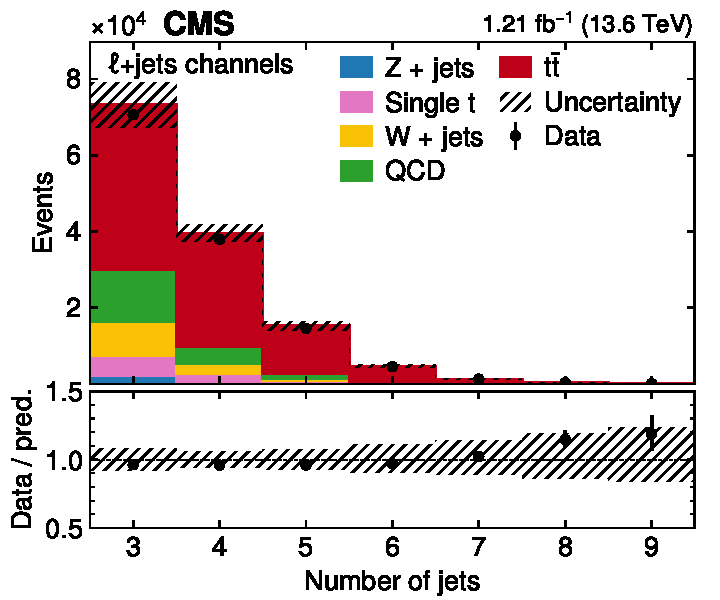
\includegraphics[width=0.49\textwidth]{figures/ttxs/njet_lj.pdf}
\hfill
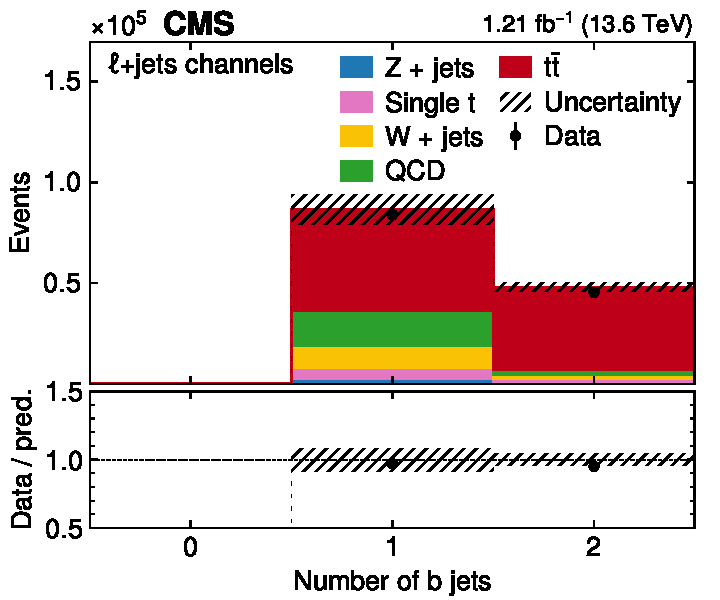
\includegraphics[width=0.49\textwidth]{figures/ttxs/nbtag_lj.pdf}
\caption{
   \textbf{Control distributions in the \ljets channels.} The distributions are shown in the same manner as in Fig.~\ref{fig:ttxs:control_em}, except for the center-right figure, which here shows \abseta of the leading jet.
}
\label{fig:ttxs:control_ljets}
\end{figure}

Good agreement between data and simulation within the full uncertainties is seen in all distributions.

\section{Likelihood fit}
\label{sec:ttxs:fit}

In order to translate the distribution of observed and expected events into a result for the inclusive \ttbar cross section while taking into account all relevant sources of systematic uncertainties, a binned profile maximum likelihood fit is used. Sec. ?? describes the setup of this fit, including the likelihood definition, while sec. ?? gives an overview of the considered systematic uncertainties and sec. ?? discusses the fit result.

\subsection{Likelihood definition}

The likelihood to be maximized in the fit is defined in terms of the \textit{signal strength} $r = \sigmatt / \sigmatt^{\text{pred}}$, i.e. the inclusive \ttbar cross section normalized to its theoretical prediction, and the \textit{nuisance parameters} $\theta_i$, which represent the different sources of systematic uncertainties. It can be written as

\begin{equation}
\label{eq:ttxs:likelihood}
    \mathcal{L} (r, \theta_i) = \prod_j \mathrm{Pois} \left(n_j^{\text{obs}} | n_j^{\text{pred}} (r, \theta_i) \right) \times \prod_i p_i ( \theta_i )
\end{equation}

where $\mathrm{Pois}$ refers to the Poisson distribution, the index $j$ runs over all bins, the observed number of events in bin $j$ is called $n_j^{\text{obs}}$, and the predicted number of events is given by

\begin{equation}
    n_j^{\text{pred}} (r, \theta_i) = r \, s_j (\theta_i) + b_j (\theta_i)
\end{equation}

with the expected number of signal and background events $s_j$ and $b_j$, respectively. 

The functions $p_i ( \theta_i )$ in eq.~\ref{eq:ttxs:likelihood} are penalty terms for the nuisance parameters $\theta_i$ and encode their pre-fit uncertainty. Two cases are present in this work: Most nuisance parameters are taken as Gaussian, in which case $\theta_i \in \mathbb{R}$ and the function $p_i ( \theta_i )$ is a Gaussian distribution with expectation value 0 and standard distribution 1. For some special cases, on the other hand, the nuisance parameters are free-floating, in which case $\theta_i \in [-1,1]$ and $p_i ( \theta_i ) = 1$. This is used mostly for the b tag scale factors, as well as the lepton scale factors in the case where no tag-and-probe method is done (compare sec.~\ref{sec:ttxs:scalefactors}).

The expected number of signal and background events as functions of the nuisance parameters are constructed from simulation and data-driven estimation using templates. For some nuisances, such as cross section uncertainties, only the total number of events is varied, which is done using a log-normal distribution, i.e. the number of background events in bin $j$ is given as

\begin{equation}
    b_j (\theta_i) = \sum_k \left(1 + \frac{\Delta\sigma_k} {\sigma_k} \right)^{\theta_k} \, n_{j,k}^{\text{pred}}
\end{equation}

where $k$ runs over all backgrounds, $\Delta\sigma_k / \sigma_k$ is the relative pre-fit uncertainty of the background cross section, and $\theta_k$ is the associated nuisance parameter. For $\theta_k = 0$, the nominal yield is recovered, while for $\theta_k = \pm 1$, the yield varies by one standard deviation.

For nuisance which might have a shape effect on the search variable, such as e.g. b tagging uncertainties, jet uncertainties or modeling uncertainties, a template morphing approach is taken: the expected distributions are calculated from simulation for a systematic variation of one standard deviation from the nominal values, and the resulting shapes are smoothly interpolated using a sixth-order polynomial. Again, $\theta_k = 0$ corresponds to the nominal shape and yield, while $\theta_k = \pm 1$ corresponds to the varied template. 

Having defined the likelihood in eq. \ref{eq:ttxs:likelihood}, the fit is carried out by maximizing the function over the signal strength and all nuisance parameters simultaneously. For numerical reasons, this is done by minimizing the negative logarithm instead. The best-fit value for $r$ is considered the final result, while the error is estimated from the resulting covariance matrix. 

\subsection{Systematic uncertainties}
\label{sec:ttxs:systematics}

% required: general shape uncertainties, special treatment of btag uncertainty, special treatment of lepton uncs in free floating case, XS uncs, lumi unc.

The systematic uncertainties considered in this work can be divided into experimental uncertainties, arising from incomplete knowledge of the details of the detector and resulting differences between data and simulation, and theoretical uncertainties, which concern imperfect modeling of the underlying physical processes in the different event generators. All of them will be described in this section.

Special attention is given to some experimental uncertainties which are important to this measurement. This includes the luminosity, which is the dominating uncertainty, as well as the lepton identification and b tagging uncertainties due to the special way they are treated in the fit.

\paragraph{Luminosity uncertainty.}

In order to translate event yields, as measured using histograms, into a result on any cross section, the total integrated luminosity is required as a calibration constant. It is immediately clear that any experimental error on the luminosity will be directly transferred to the total error on the measurement, and thus minimizing the luminosity uncertainty is crucial for any cross section mesurement.

For the dataset used in this analysis, the total luminosity uncertainty was evaluated by CMS to be 2.3\%. Of this figure, $2.1 \%$ is due to the calibration of the integrated luminosity, using the methods presented in \citere{CMS:LUM-17-003}. The largest contribution comes from factorization bias, which arises in the van der Meer method from the assumption that the transverse luminous area factorizes in the $x$ and $y$ coordinates, and from residual beam position deviations.

The agreement in the absolute scale is checked by comparing different independently calibrated luminosity measurements, and the integrated luminosity measured with the HF and the silicon pixel detector is found to agree at a level of better than 0.8\%.
Taking additional contributions due to residual differences in the time-stability and linearity between the luminosity detectors into account, leads to the full figure of 2.3\%.
A cross-check of the integrated luminosity using the yield of reconstructed Z bosons decaying into pairs of muons~\cite{CMS:DP-2023-003}, corrected for efficiencies and normalized to the fiducial cross section prediction calculated at NNLO with next-to-NNLL corrections applied, shows good agreement as well.\footnote{Since publication of this result, a more precise luminosity measurement for 2022 data has become available in \citere{CMS:LUM-22-001-PAS}.}

In contrast to all other uncertainties described below, the uncertainty in the integrated luminosity is not included in the fit, but treated as an external uncertainty and added in quadrature afterwards, since it is expected to factorize completely from all other uncertainties.
The impact of varying the normalization of the backgrounds estimated from simulation by the integrated luminosity uncertainty was found to be negligible.
% TODO.

\paragraph{b tagging uncertainty.}

As already mentioned in sec. \ref{sec:ttxs:scalefactors}, the efficiency for correctly identifying a jet originating from a b quark (b tagging) is expected to be different in data and simulation. At the time of this measurement, directly after the start of Run 3, no general-purpose b tagging studies had been available. Thus, the approach adopted here is to consider the b tagging efficiency in data to be completely unknown and measure it concurrently with the cross section in the likelihood fit.

For this purpose, the probability for an event with $n_{\mathrm{jet}}$ selected jets to have $n_{\mathrm{b tag}}$ correctly identified b jets, depending on the assumed b tagging efficiency $\epsilon_b$, is assumed to be a multinomial of the form

\begin{equation}
\label{eq:ttxs:btags}
    P (n_{\mathrm{b tag}} | n_{\mathrm{jet}}) \propto \epsilon_b^{n_{\mathrm{b tag}}} (1 - \epsilon_b)^{n_{\mathrm{b jet}}^{\mathrm{true}} - n_{\mathrm{b tag}}}
\end{equation}

Here, $n_{\mathrm{b jet}}^{\mathrm{true}}$ is the number of truth-level b jets in the event falling into the acceptance of the selection, taken from MC simulation. Note that this might be lower then the number of b jets expected from the physical process (e.g. 2 for \ttbar). 

By taking the ratio of eq. \ref{eq:ttxs:btags} in data and simulation, one can derive a scale factor for each event such that the correct distribution for the number of b tagged jets in data is reproduced. From this, a shape template depending on $\epsilon_b$ in data is constructed and included in the fit as a nuisance parameter. It can be seen in Fig. ??.

Note that any dependence of $\epsilon_b$ on the jet kinematics is integrated out in this process. Possible dependencies of the ratio of $\epsilon_b$ in data and simulation are neglected; since no kinematic information is used in the fit, this is deemed acceptable.

\paragraph{Lepton identification uncertainty.}

% TODO: the structure is kinda shit here - scale factors + uncertainty + cross check. maybe try to merge some of these?

The uncertainty assumed on the lepton identification scale factors comes from two different sources: First, an inherent uncertainty originating in the tag-and-probe method (as described in sec. \ref{sec:ttxs:scalefactors}) is considered, consisting of statistical uncertainties from both data and simulation, a systematic uncertainty derived from a comparison with a different Z+jets simulation sample produced at NLO in QCD, and another systematic uncertainty due to the choice of fitting function. Together, they make up for a X \% uncertainty on the lepton scale factors.

Secondly, it is taken into account that the scale factor between data and simulation might be slightly different in the Z+jets selection used for the T\&P method and the \ttbar selection used for the measurement of the cross section. The most important reason for this is the requirement of (b tagged) jets in almost all considered categories, as well as the requirement for at least three jets in the lepton+jets channels. 

This effect has been studied at CMS in the past and the difference found to be less then 0.5 \% for muons and 1.0 \% for electrons [??]. Taking a conservative approach, these values are used as an additional component in the respective uncertainties.

\paragraph{Pileup uncertainty.}

As described in sec. \ref{sec:ttxs:scalefactors}, three different pileup-related variables are employed to reweight the simulation to the observed data, and the average of the three weights is used as the nominal value. To assign an error to this method, it is repeated using only one of the variables - the number of good reconstructed vertices - and the difference in expected yields treated as an uncertainty. It should be noted that this difference was found to be larger then the more common method of estimating pileup-related uncertainties, which consists of deriving a theoretical expectation for the number of interactions depending on the total inelastic proton-proton cross section, and varying this number by its experimental uncertainty [??].

\paragraph{Jet energy uncertainties.}

Uncertainties in the jet energy calibration are split into 26 different sources concerning different experimental and theoretical effects, following the standard CMS procedure outlined in Ref. \cite{CMS:JME-13-004}. 17 of these sources are found to be non-negligible and included in the fit. These sources include, among others, uncertainties due to jet \pt resolution and jet flavour composition, statistical uncertainties in the derivations of the energy corrections, and residual differences between data and simulation.

\paragraph{Trigger uncertainties.}

Since the trigger scale factors are derived using the tag-and-probe method in the same way as the lepton scale factors, similar uncertainties are applied, including the extrapolation uncertainties of 0.5 \% for muons and 1.0 \% for electrons. The only difference is that, in the dilepton channels, the uncertainties need to be propagated according to eq. \ref{eq:ttxs:triggersf}. This has the effect of greatly reducing the impact of the trigger uncertainties in those channels compared to the lepton ID uncertainties, since the nominal per-event trigger efficiency is already very close to one.

\paragraph{Matrix element scale uncertainties.}

The theoretical predictions of both signal and background are calculated using matrix elements (MEs) at either leading (LO) or next-to-leading order (NLO) in perturbative QCD, matched to a parton shower (PS). Since this effectively means truncating the perturbative expansion of the scattering amplitude at a given power in the strong and electroweak coupling constants, the effect of higher-order terms is neglected in the calculation.

At the same time, the necessity of renormalization of divergent diagrams and factorization of non-perturbative contributions introduces non-physical parameters into the prediction in the form of the renormalization and factorization scales $\mu_R$ and $\mu_F$. These parameters are usually set to typical energy scales of the considered process, and might also depend on the event kinematics (dynamic scales).

To estimate possible errors due to these missing terms as well as arbitrary choices, the scales $\mu_R$ and $\mu_F$ are varied separately by a factor of 2 up and down, and the resulting change in simulation is taken as an uncertainty in the form of shape templates \cite{Cacciari:2004}. In order to not double-count uncertainties in the cross section prediction for the backgrounds (see below), but keep possible rate variations due to acceptance effects, the templates are normalized to the nominal cross section values before any selection cuts are applied. Different physical processes are considered to be uncorrelated since they are produced with different generators and at different orders. 

\paragraph{PDF uncertainties.}

In the same vein as for the matrix element uncertainties, the parton distribution functions (PDFs) used to evaluate the non-perturbative contribution of the proton-proton collision have systematic uncertainties attached. They are estimated by independently reweighting the simulation to 100 different replicas of the used NNPDF 3.1 PDF set and taking the envelope of the resulting changes, following the recommendations of the PDF4LHC working group \cite{Butterworth:2015oua}. Additionally, the effect of the choice of the strong coupling constant in the PDF is assessed using a similar reweighting. Analogously to the matrix element uncertainties, the resulting variations are normalized before any selection cuts to keep acceptance and shape effects while not double-counting cross section changes.

\paragraph{Parton shower uncertainties.}

Furthermore, the parton shower model used for the predictions has a heuristic basis and thus requires appropriate uncertainties. To retrieve these, the scales at which the strong coupling constant is evaluated are varied up and down by a factor 2 separately for initial and final state radiation, and the resulting changes propagated to the fit as a shape template.

\paragraph{ME/PS matching uncertainty.}

For the simulation of the \ttbar signal, an additional uncertainty concerning the matching between matrix element simulation in \powheg and parton showering in Pythia is considered. This is done by varying the $h_{\mathrm{damp}}$ parameter in \powheg controlling the amount of radiation generated at matrix element level, following Ref. \cite{CMS:TOP-16-021}.

\paragraph{Background cross section uncertainties.}

For the cross sections of the different processes, log-normal rate uncertainties are assigned based on the process and order at which it was calculated. Specifically, a 15 \% uncertainty is used for the single-t background since it is generated fully at NLO with a NNLO prediction for the cross section, while uncertainties of 20 \% and 30 \% are used for Z+jets as well as W+jets and Diboson, respectively, since these samples are only generated at LO. Additionally, for the fully data-driven QCD background, two separate nuisance parameters for the electron+jets and muon+jets channels are defined, covering a conservative uncertainty of 30 \% each.

\paragraph{Background statistical uncertainties.}

Finally, since the background in this measurement is estimated either using MC simulation or data-driven methods, an independent statistical uncertainty needs to be attached to each bin, reflecting the finite number of events it contains. This is done using the method given in Ref.~\cite{Barlow:1993dm}. For MC backgrounds, these uncertainties are minuscule; however, they are non-negligible for the data-driven QCD background due to the limited data statistics used there.

\subsection{Fit results}
\label{sec:ttxs:fitresults}

Performing the fit yields a \ttbar signal strength of $r = 0.958 \pm 0.025$, where the uncertainty includes statistical and all systematic contributions, except for the 2.1 \% uncertainty on the luminosity. This corresponds to an inclusive \ttbar cross section of

\[
    \sigmatt = 882 \pm 23 \, \text{(stat.+syst.)} \pm 20 \, \text{(lumi.)} \, \text{pb}
\]

The result is in agreement within one standard deviation with the standard model prediction of $\sigmatt^{\text{pred}} = 921^{+29}_{-37} \, \text{pb}$.

\begin{figure}[!p]
\centering
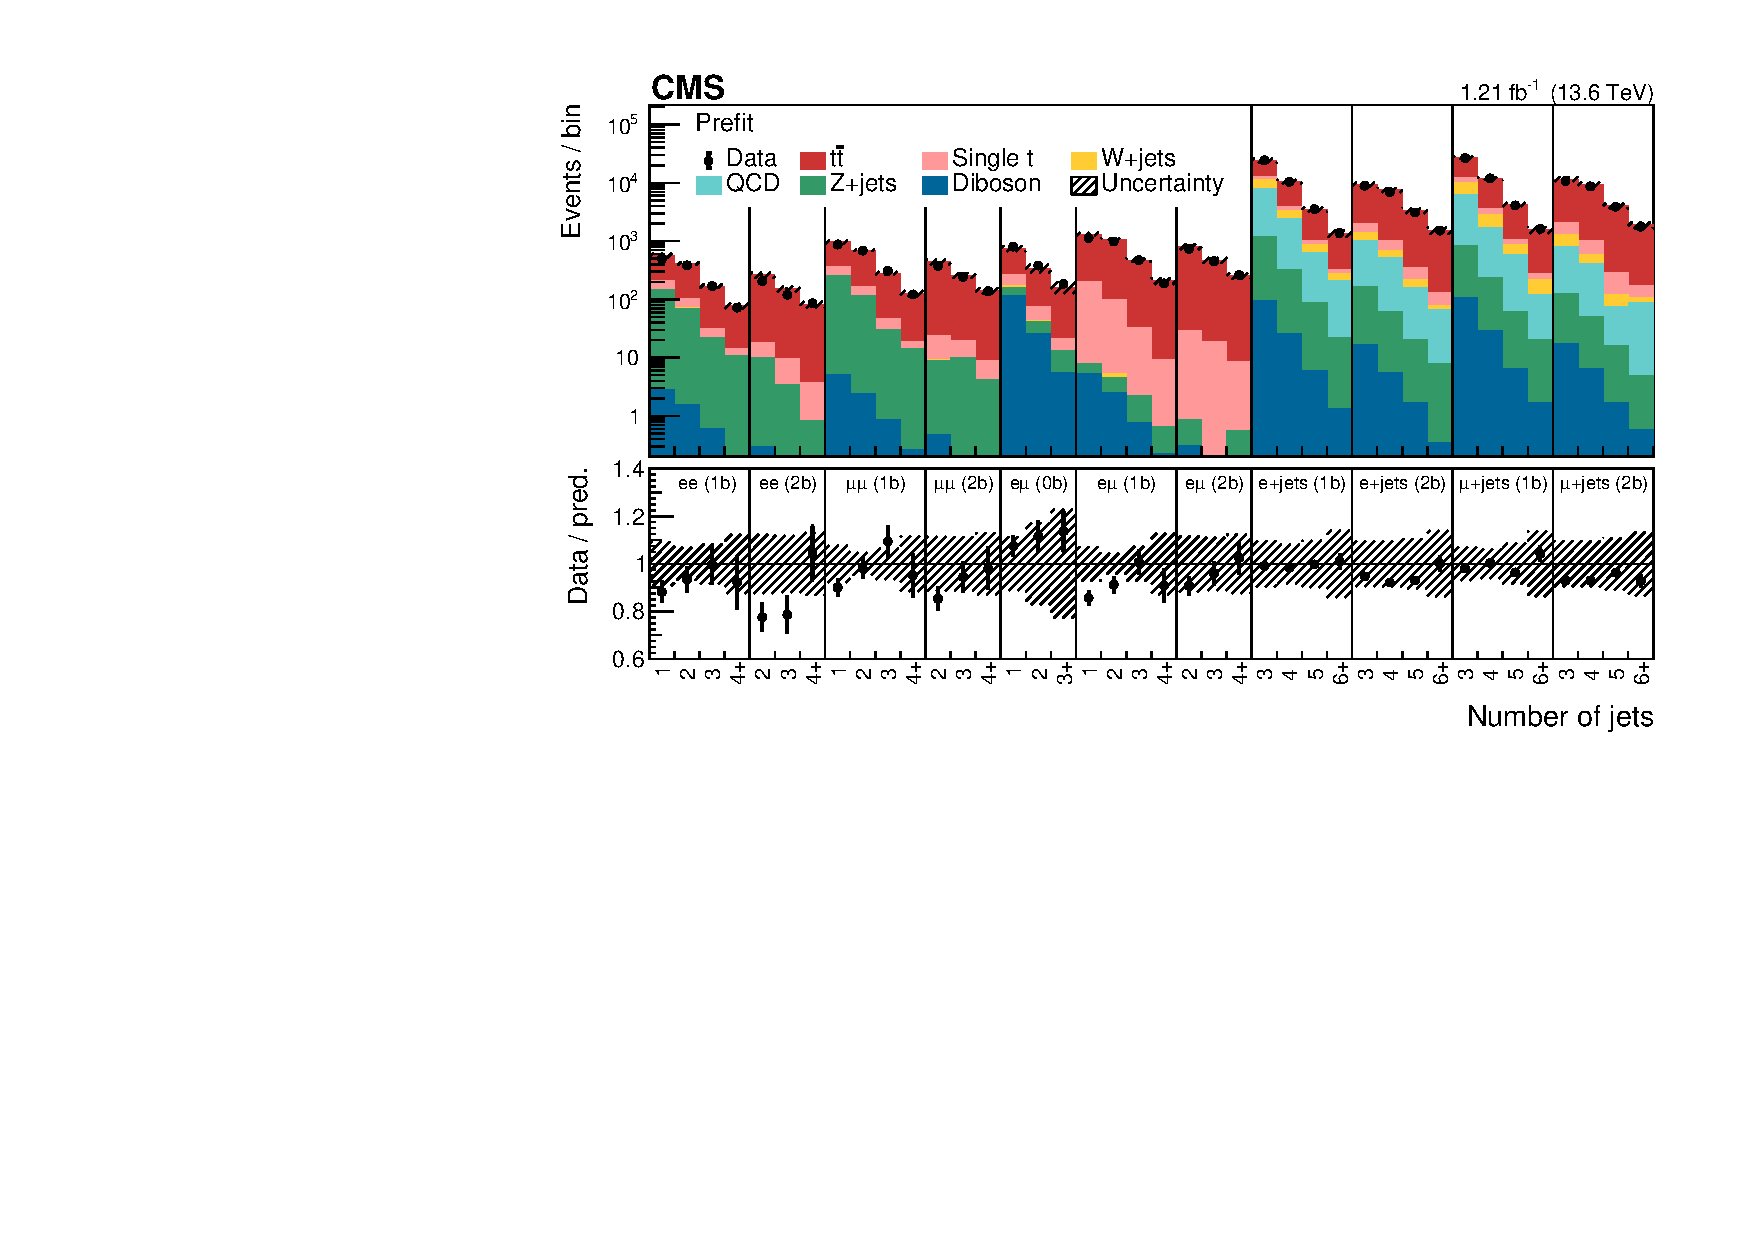
\includegraphics[width=\textwidth]{figures/ttxs/prefithist.pdf}
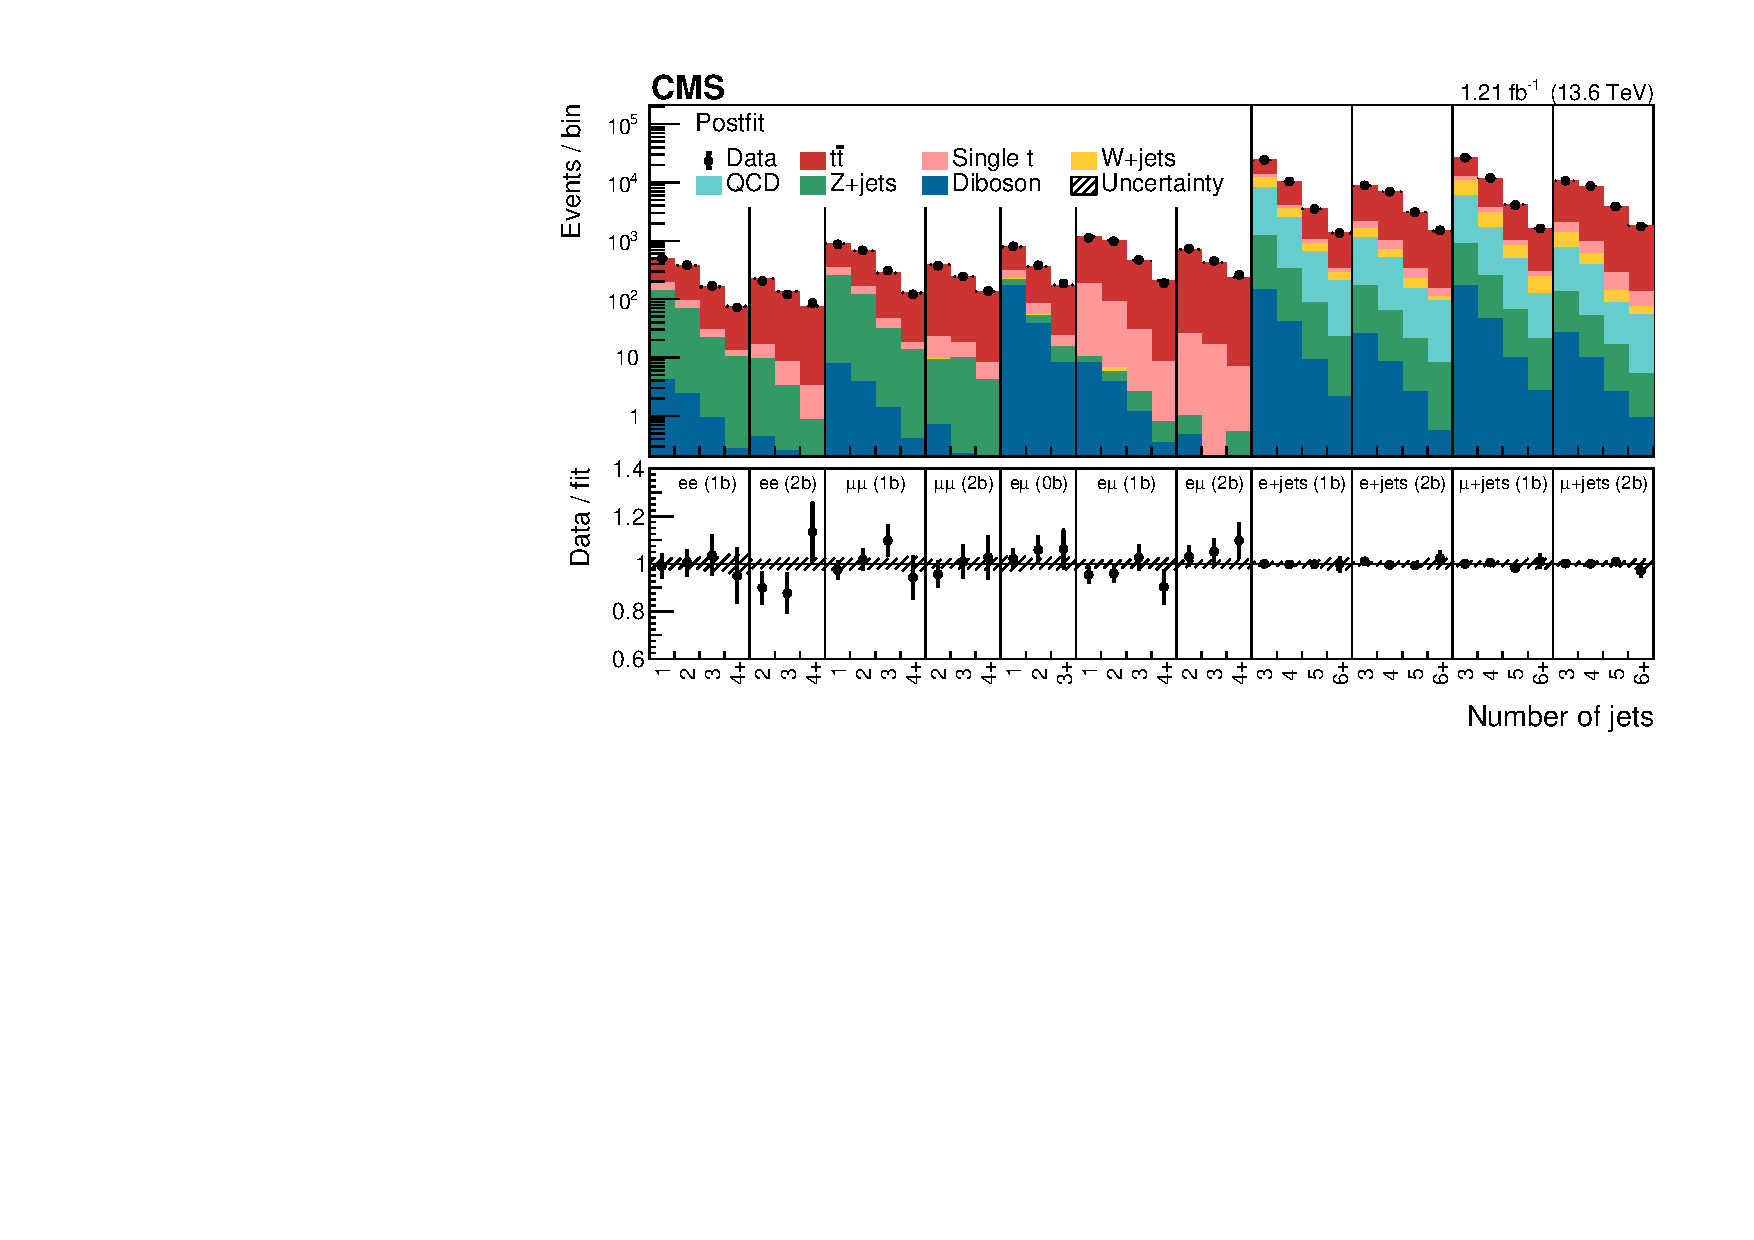
\includegraphics[width=\textwidth]{figures/ttxs/postfithist.pdf}

\caption{
   \textbf{Comparison of data and simulation before and after the fit.} The distribution of the number of jets in the different fit categories is shown for data and simulation before (top) and after the likelihood fit (bottom). The fit greatly improves the agreement and strongly constrains the background uncertainties.
}
\label{fig:ttxs:prepostfit}
\end{figure}

Fig.~\ref{fig:ttxs:prepostfit} shows the agreement between data and simulation before and after the fit. It can be immediately seen that the fit greatly reduces the uncertainty on the prediction by constraining systematic uncertainties and simultaneously improves the agreement compared to the data. 

Of particular note here is the free-floating b tagging efficiency (compare sec.~\ref{sec:ttxs:systematics}), whose effect can be directly read off from the categorization in the number of b jets: Before the fit (Fig.~\ref{fig:ttxs:prepostfit} top), the event yield for two or more b jets is overestimated in the simulation, while the yield for zero b jets is underestimated. This suggests that the b tagging efficiency is slightly lower in the data than assumed in the simulation. Indeed, the fit confirms this: the ratio of the efficiency between data and simulation in the phase space of this measurement is measured to be $\epsilon_b^{\mathrm{data}}/\epsilon_b^{\mathrm{MC}} = 0.980 \pm 0.009$. As a result, after the fit (Fig.~\ref{fig:ttxs:prepostfit} bottom), the event yields agree in all b jet categories.

To better understand the sources of systematic uncertainty, as well as the contributions of the different measurement channels, the fit is repeated twice, restricted to the dilepton and the \ljets channels, respectively. For all three cases, the contribution of different groups of nuisance parameters is calculated as explained in ??. The results can be found in Tab. ??.

\begin{table}[!htb]
\centering\renewcommand\arraystretch{1.1}
\begin{tabular}{l@{}c c c}
    Source & Full measurement & dilepton only & \ljets only\\
    \hline
    Lepton ID efficiencies & 1.6 & 2.4 & 1.0 \\
    Trigger efficiency & 0.4 & 0.0 & 0.5 \\
    JES & 0.7 & 0.7 & 1.0 \\
    b tagging efficiency & 1.0 & 0.4 & 1.8 \\
    Pileup reweighting & 0.5 & 0.0 & 1.0 \\
    ME scale, \ttbar & 0.5 & 0.4 & 0.6 \\
    ME scale, backgrounds & 0.1 & 0.1 & 0.3 \\
    ME/PS matching & 0.2 & 0.2 & 0.4 \\
    PS scales & 0.4 & 0.9 & 0.6 \\
    PDF and \alphas & 0.3 & 0.4 & 0.4 \\
    Single t background & 1.1 & 1.2 & 0.8 \\
    Z+jets background & 0.3 & 0.1 & 0.0 \\
    W+jets background & 0.0 & 0.0 & 0.1 \\
    Diboson background & 0.4 & 0.4 & 0.0 \\
    QCD multijet background & 0.3 & 0.0 & 0.5 \\
    Statistical uncertainty & 0.5 & 1.2 & 0.5 \\ \hline
    Combined uncertainty & 2.6 & 3.3 & 3.0 \\ \hline
    Integrated luminosity & 2.3 & 2.3 & 2.3 \\
\end{tabular}
\caption{
    \textbf{Sources of systematic uncertainty.} The relative per-cent contribution of different groups of sources of systematic uncertainty for the full measurement as well as for restrictions to the dilepton and \ljets channels only. They are calculated according to ?? and do not take correlations between the different groups into account.
}
\label{tab:ttxs:systematics}
\end{table}

% todo: impacts and GOF
% lepton SF consistency check
% tt curve

\section{Summary}

% what about outlook to higher lumi values? easy to do...